\section{Messungen mit Audio Precision (System Two Cascade)}
\subsection{Messung des Quantisierungsrauschens}
\subsubsection{Aufgabenstellung}
Messung des Quantisierungsrauschens (SNR) am Mischpult D/A Umsetzer (Line Ausgang des Lawo $MC^266$) mit $14-20$Bit Auflösung, Schrittweite 1 Bit. Vergleichen Sie mit den erwarteten Werten. Was kann aus den Messergebnissen gefolgert werden?

\subsubsection{Messaufbau}
Der Messaufbau dieser Übung bestand aus einem PC, der mit einer Audio Precision SYS-2722 kommunizierte und die Messsignale generierte. Am digitalen Ausgang des SYS-2722 wurde die Digital-zu-Analogkonverterkarte 941/83 des Lawo MC$^2$66 Mischpultes angeschlossen. Das analoge Signal wurde wieder in das SYS-2722 eingespeist und dort mit Hilfe der Audio Precision AP2700 Software weiterverarbeitet.
\subsubsection{Formeln}
Der Signal-Rauschabstand (SNR) aufgrund der Wortbreite $k$ lässt sich berechnen durch 
\begin{equation}
\label{form:SNR2}
SNR \ = \ 20 \ log \left(2^k\right) = 20 \cdot k \cdot log \left( 2 \right) = 6.02 \ k
\end{equation}
\subsubsection{Berechnungsbeispiele}
Bei einer Wortbreite von $k=14$ Bit (1. Zeile der Tabelle \ref{tab:snrthd}) ergibt sich das SNR zu
\begin{equation}
\label{eg:SNR8bit2}
SNR \ = \ 20 \ log \left(2^{14}\right) = 20 \cdot 14 \cdot log \left( 2 \right) = 6.02 \cdot 14 = 84.28 \text{dB}
\end{equation}
\subsubsection{Tabellen}
\begin{table}[h!]
  \begin{center}
    \begin{tabular}{ c  c c }
    \toprule
    Wortbreite &THD+N & SNR$_{berechnet}$\\
    Bit &dBr A & dB  \\ \midrule
    14 & 	90 & $84.24$  \\
    15 & 	$95.44$ & $90.3$  \\
    16 & 	$101.09$ & $96.32$  \\
    17 & 	$105.15$ & $102.34$  \\
    18 & 	$107.52$ & $108.36$  \\
    19 & 	$108.35$ & $114.38$  \\
    20 & 	$108.48$ & $120.4$  \\
    21 & 	$108.86$ & $126.42$  \\
    22 & 	$108.93$ & $132.44$  \\
    23 & 	$108.94$ & $138.5$  \\
    24 & 	$108.95$ & $144.5$  \\ \bottomrule
    \end{tabular}
  \end{center}
  \caption{Ergebnisse der Messung des THD+N und des dazugehörigen berechneten SNR.}
  \label{tab:snrthd}
\end{table}
\clearpage
\subsubsection{Diagramme}

\begin{figure}[h!]
\centering

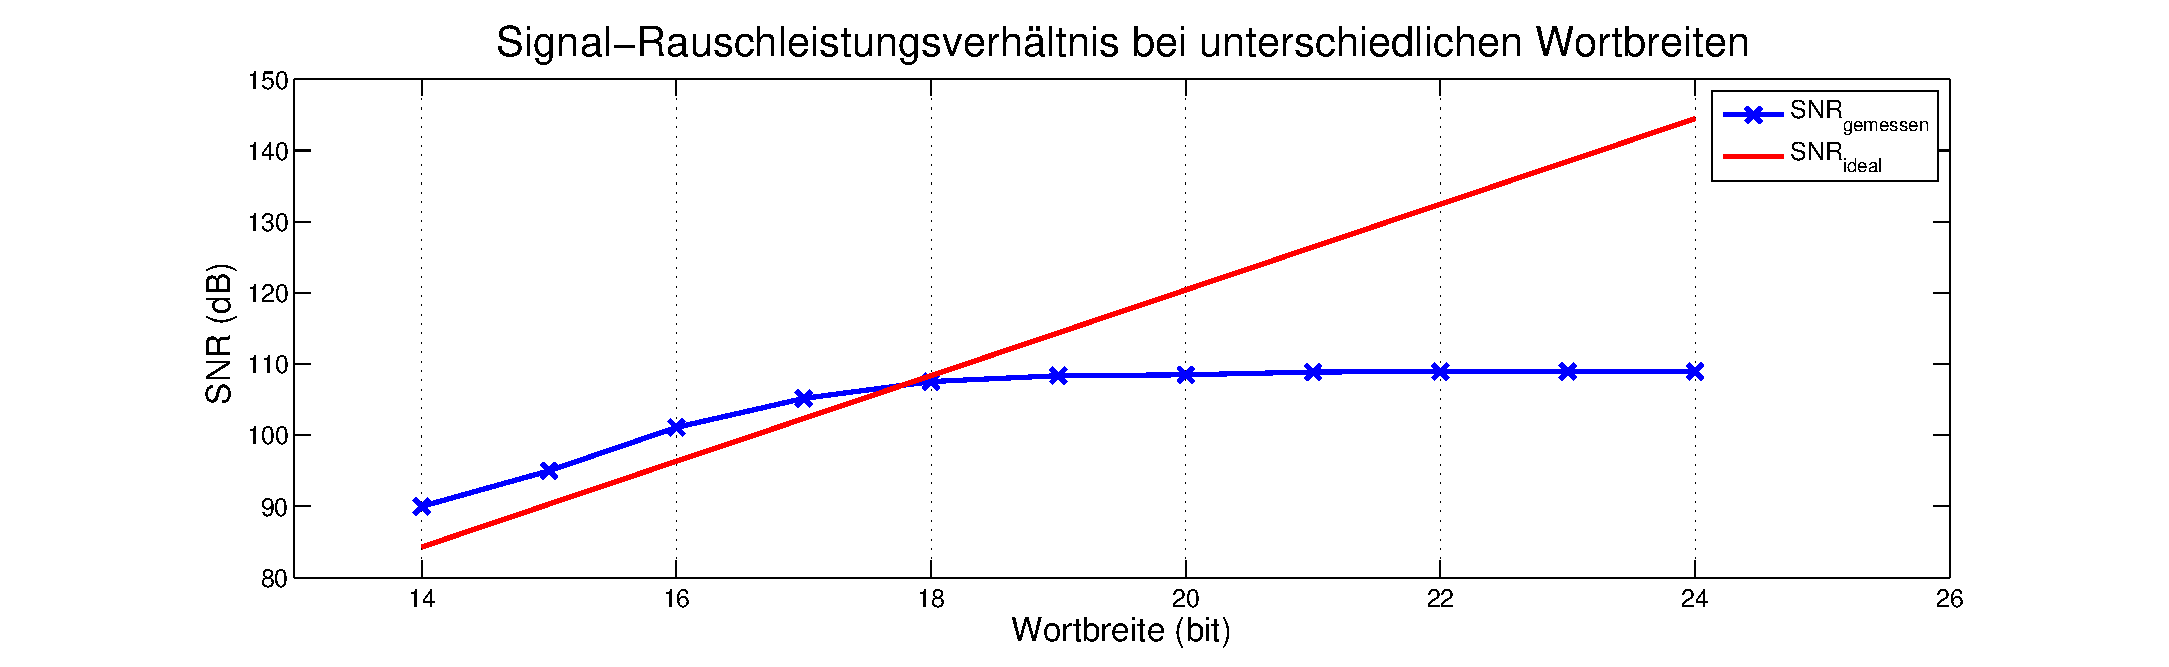
\includegraphics[width=\columnwidth]{figures/snr_wortbreite.eps} 
\caption{Vergleich des gemessenen SNR mit dem idealen SNR, bei verschiedenen Wortbreiten.}
\label{fig:d1}
\end{figure}

\subsubsection{Diskussion}
Bei dieser Teilübung wurde das SNR für verschiedene Wortbreiten aufgenommen. In Abbildung \ref{fig:d1} wird die reale der idealen Kennlinie gegenübergestellt. Wie daraus zu erkennen ist, ist im realen System die Auflösung mit 18 Bit begrenzt, da der analoge Teil der Messschaltung (Verstärker, Anpassungsnetzwerk, Aliasingfilter) für eine Limitierung sorgen.
\pagebreak


\subsection{Messung mit Jitter}
\subsubsection{Aufgabenstellung}
\begin{enumerate}
\item Messung der FFT-Spektren verjitterter Signale. Untersuchung für verschiedene Jitterfrequenzen.
\item Vergrößerung der Jitteramplitude, bis die Übertragung zusammenbricht.
\item Aufzeichnung der THD+N - Kennlinie bei den Jitterfrequenzen $500$Hz, $5$kHz und $10$kHz. 
\end{enumerate}


\subsubsection{Messaufbau}
Der Messaufbau der ersten Übung wurde modifiziert. Da das MC$^2$66 zu gut ist, wurde es durch das Fireface UFX ersetzt.

\subsubsection{Formeln}
Bei dieser Teilübung war nichts zu berechnen.
\subsubsection{Berechnungsbeispiele}
Es wurden keine Berechnungen durchgeführt.

\subsubsection{Diagramme}

\begin{figure}[h!]
\centering
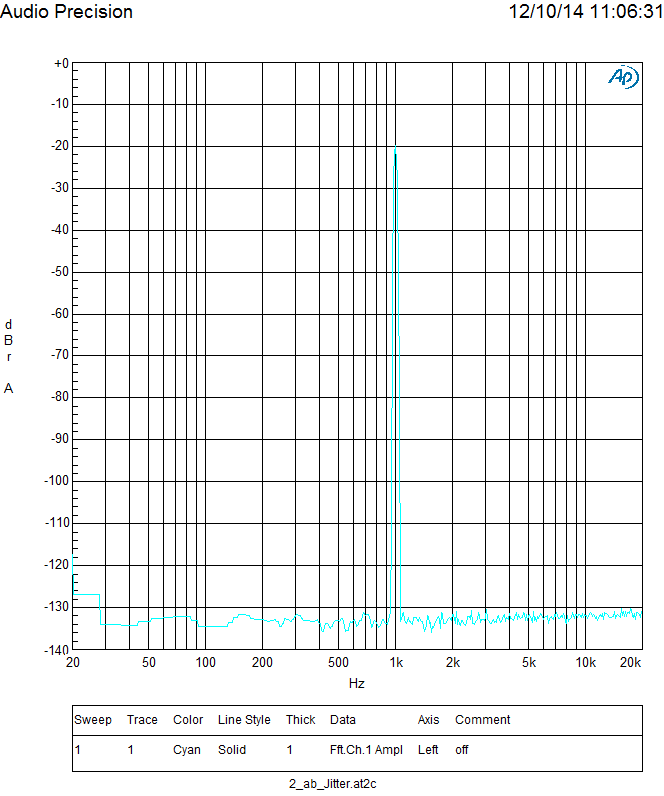
\includegraphics[width=\columnwidth]{figures/Aufg2/off_1khz.PNG} 
\caption{THD+N Kennlinie über die Frequenz bei einem Sinus von 1 kHz.}
\label{fig:1}
\end{figure}


\begin{figure}[h!]
\centering
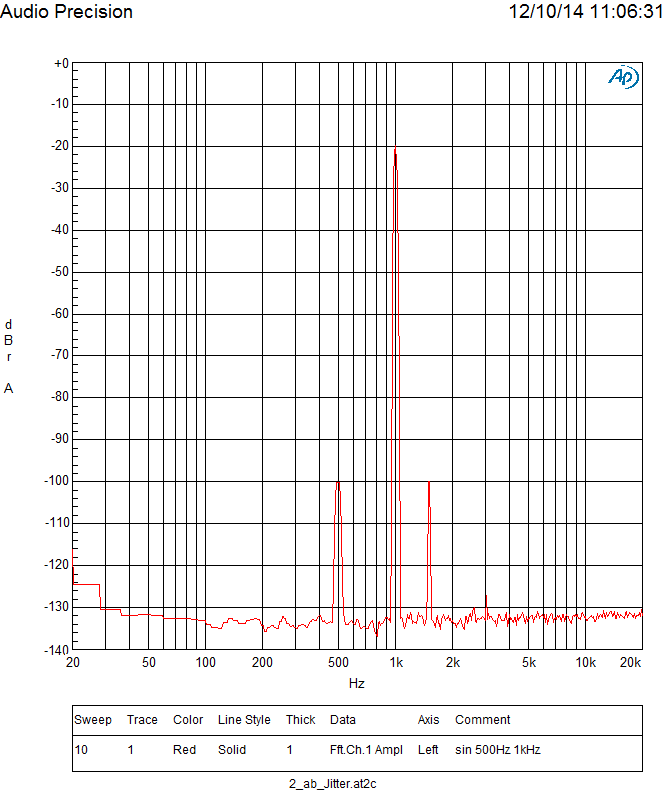
\includegraphics[width=\columnwidth]{figures/Aufg2/10.PNG} 
\caption{THD+N Kennlinie über die Frequenz bei einem Sinus von 1 kHz und einer sinusförmigen Jitterfrequenz von 500 Hz.}
\label{fig:2}
\end{figure}

\begin{figure}[h!]
\centering
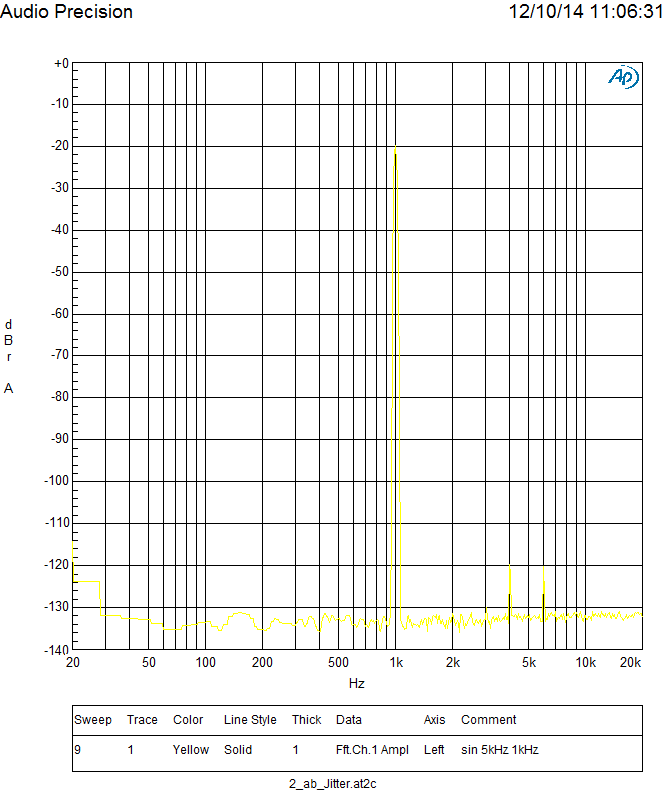
\includegraphics[width=\columnwidth]{figures/Aufg2/9.PNG} 
\caption{THD+N Kennlinie über die Frequenz bei einem Sinus von 1 kHz und einer sinusförmigen Jitterfrequenz von 5000 Hz.}
\label{fig:3}
\end{figure}

\begin{figure}[h!]
\centering
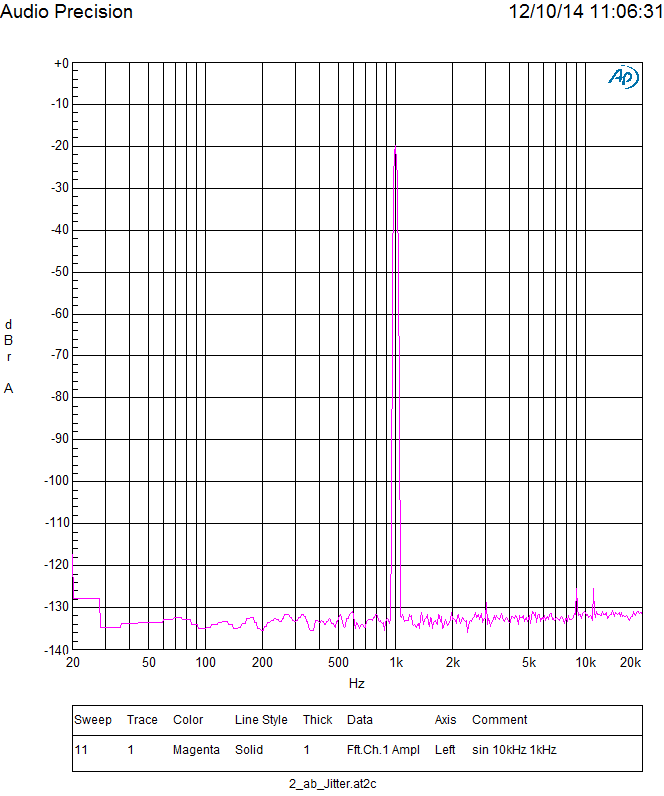
\includegraphics[width=\columnwidth]{figures/Aufg2/11.PNG} 
\caption{THD+N Kennlinie über die Frequenz bei einem Sinus von 1 kHz und einer sinusförmigen Jitterfrequenz von 10000 Hz.}
\label{fig:4}
\end{figure}


\begin{figure}[h!]
\centering
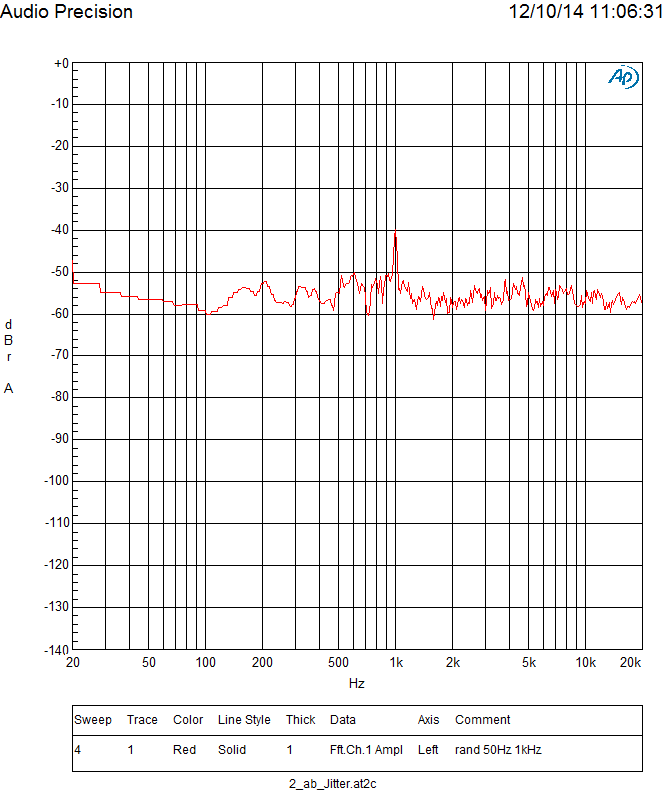
\includegraphics[width=\columnwidth]{figures/Aufg2/4.PNG} 
\caption{THD+N Kennlinie über die Frequenz bei einem Sinus von 1 kHz und einer randomisierten Jitterfrequenz von 50 Hz.}
\label{fig:5}
\end{figure}
\clearpage

\subsubsection{Diskussion}
Zunächst wurden mit Hilfe des Aufbaues die Abbildungen (\ref{fig:1} bis \ref{fig:4}) aufgenommen. Hierbei wurde ein sinusförmiger Jitter und ein 16 faches Average eingestellt. Bei Abbildung \ref{fig:2} erkennt man, dass sich Seitenbänder um 500 Hz, links und rechts um die Grundfrequenz ausbilden. Dies tritt auf, da ein sinusförmiger Jitter mit 500 Hz verwendet wird und das Spektrum sich wie das einer Frequenzmodulation verhält. Bei Abbildung \ref{fig:3} wurde ein sinusförmiger Jitter mit 5000 Hz verwendet. Bei 6000 Hz tritt wie zu erwarten ein Seitenband auf (5 kHz + 1 kHz). Der Peak bei 4 kHz ist mit der Spiegelung des zweiten Seitenbandes von -4 kHz (1 kHz - 5 kHz) zu erklären. Bei Abbildung \ref{fig:4} tritt das selbe Phänomen auf (sinusförmiger Jitter mit 10 kHz).
\\
Danach wurde der Jitter auf randomisiert gestellt. Trotz größtmöglicher Jitteramplitude und randomisierten Jitter ist der Peak bei 1 kHz gut zu erkennen. Dies geht aus Abbildung \ref{fig:5} hervor. Somit war es nicht möglich die Übertragung zu verhindern.

\subsection{Klirrfaktor}
\subsubsection{Aufgabenstellung}
\begin{enumerate}
\item Messen einer THD+N-Kennlinie über den Dynamikbereich mit und ohne Dither
\item Messen einer THD+N-Kennlinie über der Frequenz mit und ohne Dither
\end{enumerate}

\subsubsection{Messaufbau}
Der Messaufbau ist der vorigen Übung zu entnehmen.
\subsubsection{Formeln}
Bei dieser Teilübung war nichts zu berechnen.
\subsubsection{Berechnungsbeispiele}
Es wurden keine Berechnungen durchgeführt.

\subsubsection{Diagramme}
\begin{figure}[h!]
\centering
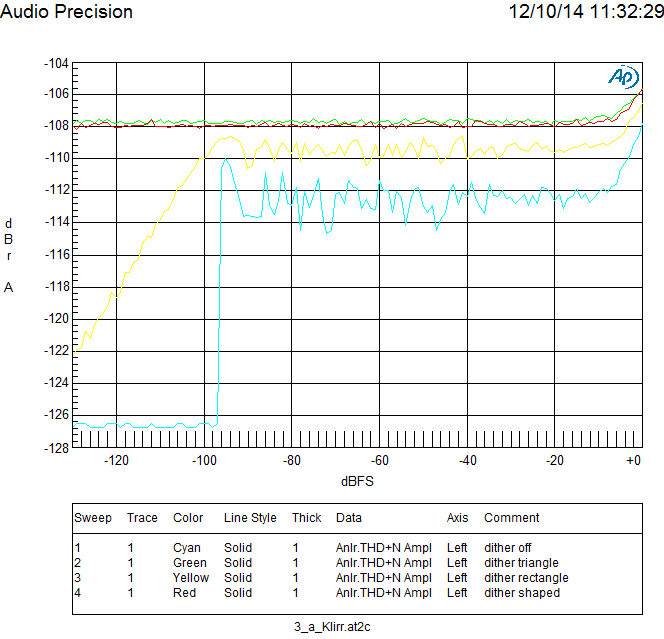
\includegraphics[width=\columnwidth]{figures/Aufg2/3a5.PNG} 
\caption{Kennlinie des THD+N über den gesamten Dynamikbereich, bei verschiedenen Dithereinstellungen}
\label{fig:100}
\end{figure}

\begin{figure}[h!]
\centering
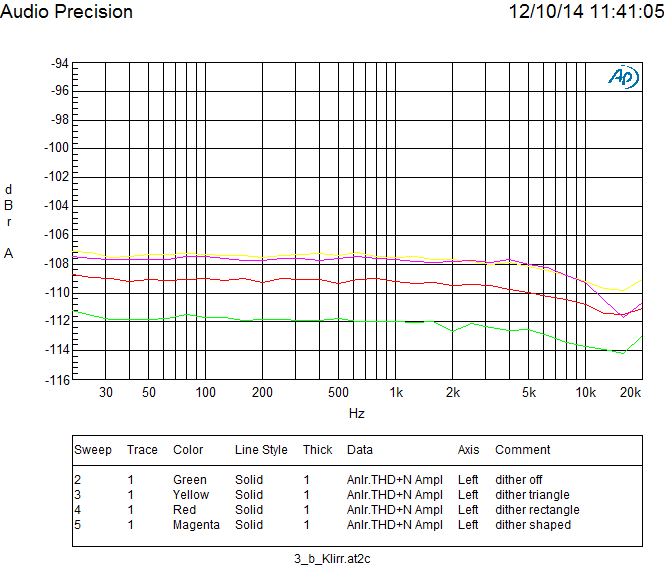
\includegraphics[width=\columnwidth]{figures/Aufg2/3b1.PNG} 
\caption{Kennlinie des THD+N über das Frequenzspektrum, bei verschiedenen Dithereinstellungen}
\label{fig:1000}
\end{figure}
\clearpage
\subsubsection{Diskussion}
Mit Hilfe der Computersoftware und einem Preset, wurde die THD+N Kennlinie über den Dynamikbereich und der Frequenz aufgenommen. Siehe Abbildungen \ref{fig:100} und \ref{fig:1000}. Aus dem Diagramm für den Dynamikbereich kann man erkennen, dass die Dynamikschwankungen mit Dither geringer werden. Weiters ist zu entnehmen, dass ohne Dither ein Einbruch auftritt, wenn die Amplitude kleiner als das LSB wird.
Der Frequenzbereich zeigt wie zur erwarten, dass ein Signal ohne Granularrauschen mit Dither ein schlechteres SNR besitzt.


\subsection{Geräteliste}
\begin{itemize}
\item PC mit Audio Precision AP2700 Software
\item Audio Precision SYS-2722
\item A/D-Wandlerkarte 941/83 des Lawo MC$^2$66
\item Fireface UFX
\end{itemize}


